\section{Инструментальная среда Opermon}

Opermon [\ref{monitoring_tools}] - инструмент для отображения, анализа и сбора трасс, созданный изначально для работы с бортовыми авиационными шинами данных, такими как MSTD-1553, ARINC, FibreChannel и CAN. На сегодняшний день Opermon имеет следующие возможности:

\begin{itemize}
 \item отображение обменов в табличном виде;
 \item сохранение трасс для последующего анализа (с возможностью удаления старых обменов из трассы для длительной непрерывной работы);
 \item разбор сообщений с выделением параметров;
 \item отображение значений параметров в табличном виде или в виде графиков.
\end{itemize}

Решение Opermon имеет клиент-серверную архитектуру, где разделены инструмент взаимодействия с адаптером и средство визуализации. 

\begin{figure}[H]
 \centering
 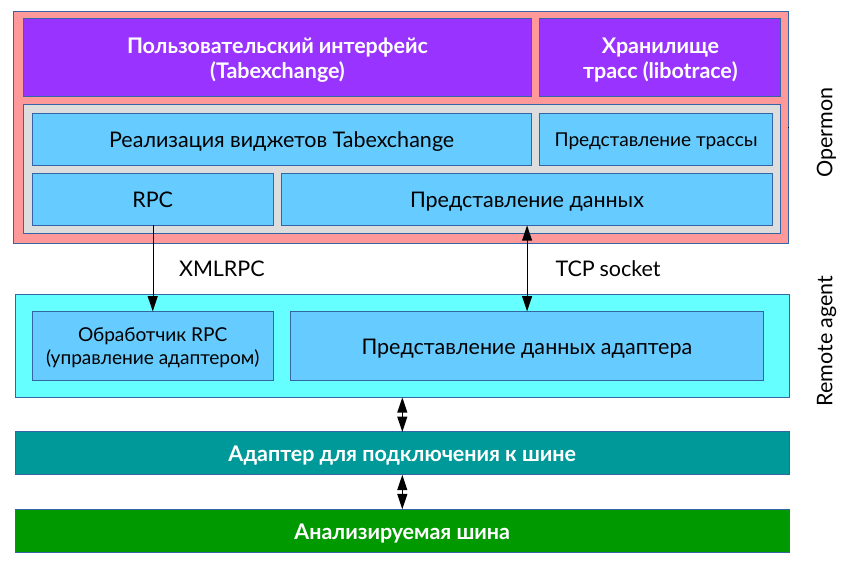
\includegraphics[width=\textwidth]{opermon_base}
 \caption{Структурная схема связи компонентов среды Opermon}
 \label{fig:opermon_base}
\end{figure}

\subsection{Серверная часть}

\label{agent_base}

Задача удалённого агента - устанавливать соединение с адаптером и обеспечивать обмен данными между адаптером и средством визуализации Opermon. Взаимодействие с Opermon происходит через пару TCP-соединений.

Первое соединение служит для передачи команд управления через RPC (Remote Procedure Call, вызов удалённых процедур) с помощью библиотеки qxmlrpc [\ref{qxmlrpc}]. Агент ожидает подключения средства визуализации.

Второе TCP-соединение открывается по команде bind от средства визуализации. Через это соединение передаются данные о прочитанных обменах, а также сообщения в очередь на передачу через адаптер (если реализация интерфейса в Opermon поддерживает передачу данных на шину).

\subsection{Клиентская часть}

Средство визуализации оформлено в виде окна с набором отделяемых виджетов для отображения данных и настройки различных параметров. 

В задачи средства визуализации также входит предоставление пользовательского интерфейса для подключения к агенту (или нескольким агентам) и для настройки параметров адаптеров.

Основное окно программы содержит следующие виджеты [\ref{sma_manual}]:

\begin{itemize}
 \item \textbf{Область отображения результатов}. В этом виджете отображается таблица обменов (несколько таблиц при использовании нескольких адаптеров), а также статистика обменов и параметры передаваемой циклограммы (если поддерживается адаптером).
 \item \textbf{Панели инструментов}. Позволяют выбирать текущие отображаемые виджеты, а также управлять текущим режимом работы анализатора.
 \item Виджеты боковой панели:
 \begin{itemize}
  \item \textbf{Настройка адаптеров}. Предоставляет интерфейс для выбора адаптеров для работы, а также позволяет настроить каждый выбранный адаптер в отдельности (с возможностью получать данные от разных агентов).
  \item \textbf{Расширенная информация о выбранном обмене}. Позволяет просматривать информацию о выбранном обмене в виде пар ключ-значение.
  \item \textbf{Фильтр обменов}. Инструмент, дающий возможность отображать и обрабатывать только те обмены, которые соответствуют выбранным параметрам.
  \item \textbf{Поиск}. Предоставляет возможность искать конкретные обмены по запросу пользователя.
 \end{itemize}
 \item \textbf{Область информационных сообщений}. Отображает список произошедших за время работы анализатора событий (таких как загрузка сессии, подключение к адаптеру, начало и конец регистрации обменов) в хронологическом порядке.
 \item \textbf{Строка состояния}. Описывает текущий режим работы анализатора.
\end{itemize}

\subsection{Инструмент хранения трасс обменов}

Средство хранения трасс позволяет пользователю производить запись трассы получаемых обменов для последующего отображения, обработки и анализа. 

Данный функционал в актуальной версии решения Opermon реализуется логическим модулем libotrace и частично в клиентской части. Доступ к функционалу предоставляется в рамках клиентской части среды.

В задачи инструмента хранения трасс обменов входят:

\begin{itemize}
 \item \textbf{Сбор и экспорт данных трасс обменов}. Трассы обменов сохраняются на диск в отчуждаемом формате. Таким образом, есть возможность анализировать обмены вне рабочего места оператора (часто собранные данные полезны разработчикам и инженерам, работающим с анализируемой системой).
 \item \textbf{Удаление устаревших данных в процессе записи трассы}. Данная функция необходима в случае длительной непрерывной работы решения, когда свободного дискового пространства может не хватить для записи всех полученных обменов. В этом случае в зависимости от настройки Opermon может удалять старые обмены в процессе записи для экономии пространства.
\end{itemize}

\subsection{Особенности архитектуры решения}

В этом разделе описаны особенности архитектуры Opermon, определяющие порядок реализации нового типа адаптера в среде.

\subsubsection{Представление данных в среде}

Для корректного представления данных в среде и для возможности адекватно их обрабатывать требуется достаточно жёсткая структуризация получаемых от адаптера данных. В среде Opermon каждый обмен имеет как минимум два основных способа представления, это связано с тем, что в текущей версии обмены обрабатываются по отдельности средством визуализации и инструментом для хранения трасс:

\begin{itemize}
 \item \textbf{Представление для инструмента отображения}. Здесь от представления требуется максимальная информативность, возможность разделения на логические поля для упрощения отображения.
 \item \textbf{Представление для инструмента хранения трасс обменов}. От представления требуется возможность сериализации данных (возможность сохранения их во внешнем файле для последующего импорта в инструмент анализа и обработки).
\end{itemize}

\subsubsection{Обмен данными между агентом и средством визуализации}

Как было описано в разделе \ref{agent_base}, между клиентской и серверной частями устанавливается два TCP-соединения: для управления адаптерами через RPC и для обмена данными (для каждого адаптера).

В RPC серверной части решения требуется реализовать набор базовых функций управления:

\label{agent_proc_list}

\begin{itemize}
 \item \textbf{list} - для получения списка доступных адаптеров данного типа;
 \item \textbf{bind} - для подключения к определённому адаптеру системы;
 \item \textbf{ping} - для периодической проверки доступности адаптера в системе во время работы;
 \item \textbf{connect} - для установки дополнительного TCP-соединения для обмена данными;
 \item \textbf{start} - для начала обмена данными с адаптером;
 \item \textbf{stop} - для остановки обмена данными с адаптером;
 \item \textbf{unbind} - для отсоединения от адаптера, что сделает его доступным для других приложений системы;
 \item \textbf{setOptions} - для чтения и установки параметров адаптера;
 \item \textbf{putData} - для передачи циклограмм обменов от клиента адаптеру (вывод данных в шину).
\end{itemize}


Формат данных для передачи обменов не стандартизирован и может быть выбран разработчиком реализации конкретного интерфейса в зависимости от особенностей анализируемой шины.

\subsubsection{Виджеты для отображения и конфигурации}

Решение Opermon разработано на базе фреймворка Qt [\ref{qt_home}] и использует его возможности для реализации графического пользовательского интерфейса.

Для стандартных виджетов Opermon подготовлены интерфейсы взаимодействия с ядром системы. Каждый из стандартных виджетов требует отдельной реализации для всех типов адаптеров.